\documentclass[a4paper,12pt, norsk]{article}
\usepackage[utf8]{inputenc}
\usepackage{graphicx}
\usepackage[norsk]{babel}
\usepackage{parskip}







\title{DB1 \\ Konseptuelt skjema: ER-modell}
\author{Fellesprosjektet: Gruppe 27 \\ Andreas Drivenes, Bjørn Bråthen, Eivind Havikbotn, \\ Nicholas Tidemand, Einar Eilertsen Eldevik, Eivind Gjerde Johansen}
\date{3. mars 2014}
\begin{document}
\maketitle

\section*{ER-modell for fellesprosjektet}

\begin{center}
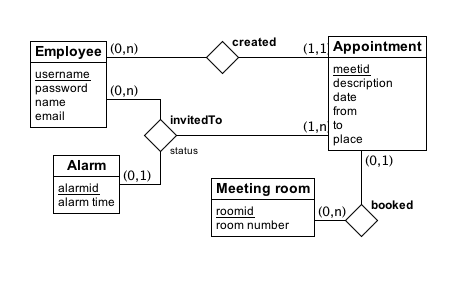
\includegraphics[width=\textwidth]{db1.png}
\end{center}
\clearpage

\section*{Oppfyllelse av kravspesifikasjonen}

\subsubsection*{1. Logge på.}

Vi har en Employee-entitet hvor brukernavnet er den unike nøkkelen. Brukeren logges på ved å oppgi rett brukernavn og passord som lagret i databasen. 

\subsubsection*{2. Legge inn avtale.}
Brukeren som lager avtalen får en relasjon til Appointment-entiteten (brukernavnet lagres i møtetabellen som en fremmednøkkel). Det opprettes også en invitedTo-relasjon der statusen settes til Attending. 

\subsubsection*{3. Håndtere møtedeltakere.}
Brukeren som inviteres får en relasjon til Meeting ved invitedTo, og status-variabelen (enum) der settes til «Pending». Deretter kan brukeren svare Not Attending eller Attending

\subsubsection*{4. Endre avtale}
Den ansvarlige brukeren for møtet kan slette et møte siden databasen kan sjekke at denne brukeren faktisk opprettet møtet. Det går an å oppdatere status-attributtet i invitedTo-relasjonen til Pending for alle møtedeltakere. Her er vi fortsatt litt usikre på hvordan vi implementere varslinger om endring. 

\subsubsection*{5. Slette avtale.}
Brukeren som opprettet avtalen sletter den. Dermed slettes også alle oppføringene i Employee-Appointment-tabellen (on cascade delete f. eks)

\subsubsection*{6. Reservere møterom.}
Dersom brukeren velger å legge til et møterom, opprettes det en relasjon mellom Meeting og Meeting room. Ved oppdatering av tidspunkt der det er en annen relasjon som har samme tidspunkt, kuttes relasjonen mellom Meeting og Meeting room.

\subsubsection*{7. Visning}
Her er det bare å hente ut all info som ligger lagret i databasen. Vi har kontroll på hvem som har opprettet møtet og hva statusen til møtedeltagerene er. 

\subsubsection*{8. Status for deltakelse}
I relasjonen invitedTo er det en status-attributt som holder styr på hvem som har svart osv. 

\subsubsection*{9. Melde avbud for møte}
Hvis avtalen blir slettet i kalenderen, oppdateres statusattributet til «Not attending» og et varsel sendes ut til alle møtedeltagere. 

\subsubsection*{12. Spore møteinnkallinger }
Dette er dekket i punkt 3. 

\subsubsection*{13. Vis flere kalendre. }
Man kan bare hente ut informasjon om flere ansattes kalendre samtidig fra databasen.

\subsubsection*{14. Alarm}
Id-en som peker på alarm blir lagret sammen med møteiden og brukernavnet. Man kan selv sette alarmtidspunkt. 

\end{document}
